\documentclass[tikz,border=10pt]{standalone}
\usepackage{amsmath}
\usepackage{tikz}
\usetikzlibrary{arrows.meta, positioning, calc, shapes.geometric}

\begin{document}
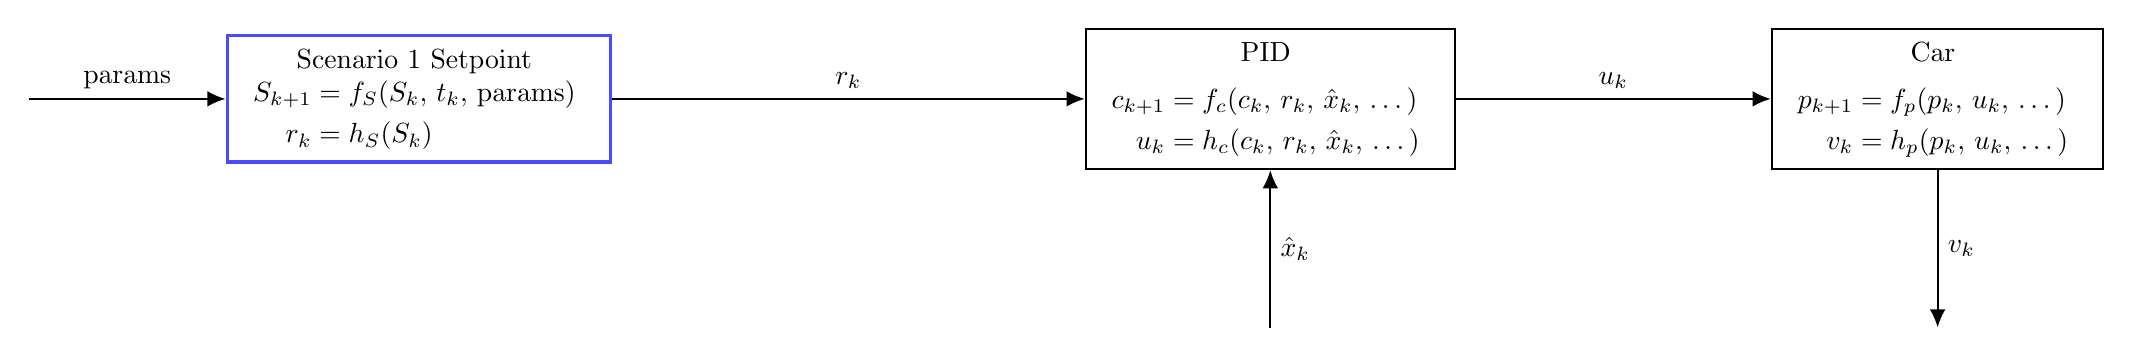
\begin{tikzpicture}[
  block/.style = {draw, thick, minimum height=3em, minimum width=6em, align=center},
  blueblock/.style = {draw=blue!70, very thick, minimum height=3em, minimum width=6em, align=center},
  arrow/.style = {thick, -{Latex[width=2mm]}},
  node distance=2.5cm and 2.5cm
]

% ======================================================
% Scenario 1 Setpoint (blue block)
% ======================================================
\node[blueblock] (setpoint) {
  \begin{tabular}{c}
    Scenario 1 Setpoint \\
    $\begin{aligned}
      S_{k+1} &= f_S(S_k,\, t_k,\, \mathrm{params}) \\
      r_k &= h_S(S_k)
    \end{aligned}$
  \end{tabular}
};

% External params arrow into Scenario 1 Setpoint
\coordinate (external_params) at ($(setpoint.west)+(-2.5,0)$);
\draw[arrow] (external_params) -- node[above] {params} (setpoint.west);

% ======================================================
% PID Controller (to the right)
% ======================================================
\node[block, right=6cm of setpoint] (pid) {
  \begin{tabular}{c}
    PID \\[0.5em]
    $\begin{aligned}
      c_{k+1} &= f_c(c_k,\,r_k,\,\hat{x}_k,\,\dots) \\
      u_k &= h_c(c_k,\,r_k,\,\hat{x}_k,\,\dots)
    \end{aligned}$
  \end{tabular}
};

% r_k arrow from Scenario 1 Setpoint to PID
\draw[arrow] (setpoint.east) -- node[midway, above] {$r_k$} (pid.west);

% Bottom input: \hat{x}_k to PID
\draw[arrow] ($(pid.south)+(0,-2.0)$) -- node[midway, right] {$\hat{x}_k$} (pid.south);

% ======================================================
% Car (Plant) Block (to the right)
% ======================================================
\node[block, right=4cm of pid.east] (plant) {
  \begin{tabular}{c}
    Car \\[0.5em]
    $\begin{aligned}
      p_{k+1} &= f_p(p_k,\,u_k,\,\dots) \\
      v_k &= h_p(p_k,\,u_k,\,\dots)
    \end{aligned}$
  \end{tabular}
};

% Single u_k arrow from PID to Plant
\draw[arrow] (pid.east) -- node[above] {$u_k$} (plant.west);
% Bottom output: v_k
\coordinate (vk_out) at ($(plant.south)+(0,-2.0)$);
\draw[arrow] (plant.south) -- node[right] {$v_k$} (vk_out);
\end{tikzpicture}
\end{document}
